\documentclass[12pt, oneside]{article} 
% \documentclass{article} 
\usepackage{amsmath, amsthm, amssymb, calrsfs, wasysym, verbatim, bbm, color, graphics, geometry}
\usepackage{fancyvrb} % for "\Verb" macro
\usepackage[toc,page]{appendix}
\usepackage[pdftex]{graphicx}
\usepackage{float}
\usepackage{hyperref}
\hypersetup{
    colorlinks=true,
    linkcolor=blue,
    filecolor=magenta,      
    urlcolor=cyan,
}
 
\urlstyle{same}

\geometry{tmargin=1.25in, bmargin=1.25in, lmargin=1.00in, rmargin = 1.00in}  

\newcommand{\R}{\mathbb{R}}
\newcommand{\C}{\mathbb{C}}
\newcommand{\Z}{\mathbb{Z}}
\newcommand{\N}{\mathbb{N}}
\newcommand{\Q}{\mathbb{Q}}
\newcommand{\Cdot}{\boldsymbol{\cdot}}

\usepackage{listings}
\usepackage{color} %red, green, blue, yellow, cyan, magenta, black, white
\definecolor{mygreen}{RGB}{28,172,0} % color values Red, Green, Blue
\definecolor{mylilas}{RGB}{170,55,241}

\title{CIS580 PSet 3}
\author{Sheil Sarda}
\date{02.24.2021}

\begin{document}
\lstset{language=Matlab,%
    %basicstyle=\color{red},
    breaklines=true,%
    morekeywords={matlab2tikz},
    keywordstyle=\color{blue},%
    morekeywords=[2]{1}, keywordstyle=[2]{\color{black}},
    identifierstyle=\color{black},%
    stringstyle=\color{mylilas},
    commentstyle=\color{mygreen},%
    showstringspaces=false,%without this there will be a symbol in the places where there is a space
    numbers=left,%
    numberstyle={\tiny \color{black}},% size of the numbers
    numbersep=9pt, % this defines how far the numbers are from the text
    emph=[1]{for,end,break},emphstyle=[1]\color{red}, %some words to emphasise
    %emph=[2]{word1,word2}, emphstyle=[2]{style},    
}

\begin{titlepage}
    \begin{flushleft}
        \vspace*{1cm}
        \Huge
        \textbf{CIS580 Problem Set 3\\ }
        \vspace*{0.5cm}
        \normalsize
        Sheil Sarda \verb|<sheils@seas.upenn.edu>| \\
        CIS580 Spring 2021
        \tableofcontents
    \end{flushleft}
\end{titlepage}

\section{Transformation to map facade to rectangle}

\clearpage
\section{Compute distances of patrol car and bridge}

\clearpage
\section{Compute distances from the image}

\clearpage
\section{Different perspectives in a tennis match}

\begin{itemize}
  \item You should get the coordinates of the points in the image. To do so you can use 
      any unit you want. Using pixels is the most convenient. 
  \item The cross ratio should  be applied in one of the baselines, and you can use 
      the net in the middle of the court as an extra point.
  \item Since you have measured coordinates of A and B, you can use the similar triangle 
      to obtain the coordinate of V.
  \item I had taken average of the vanishing points obtained by using cross ratio on AB 
      and CD due to the minor differences between them.
  \item For each pair of sidelines you should find 1 vanishing point (so 2 in total 
      for the two images). In the same image using the cross ratio in the two sidelines, 
      you  should get the same vanishing points (they will not be exactly the same but 
      they will be close enough, you can just use one of them)
  \item For the intersection of baselines you can use intersection of lines.
  \item You cannot define a coordinate system where (0,0,1) is one corner and (1,1,1) 
      is the other because you will mess the distances. In the tennis case we don't 
      have a square. You should modify the method so that it uses [27,78,1] 
      instead of [1,1,1]
  \item  Oh, I see. We should use two images of the same plane, tennis court, to construct 
      two vanishing lines and find the principle point.
\end{itemize}


\subsection{Why is the perspective different}

\begin{figure}[H]
  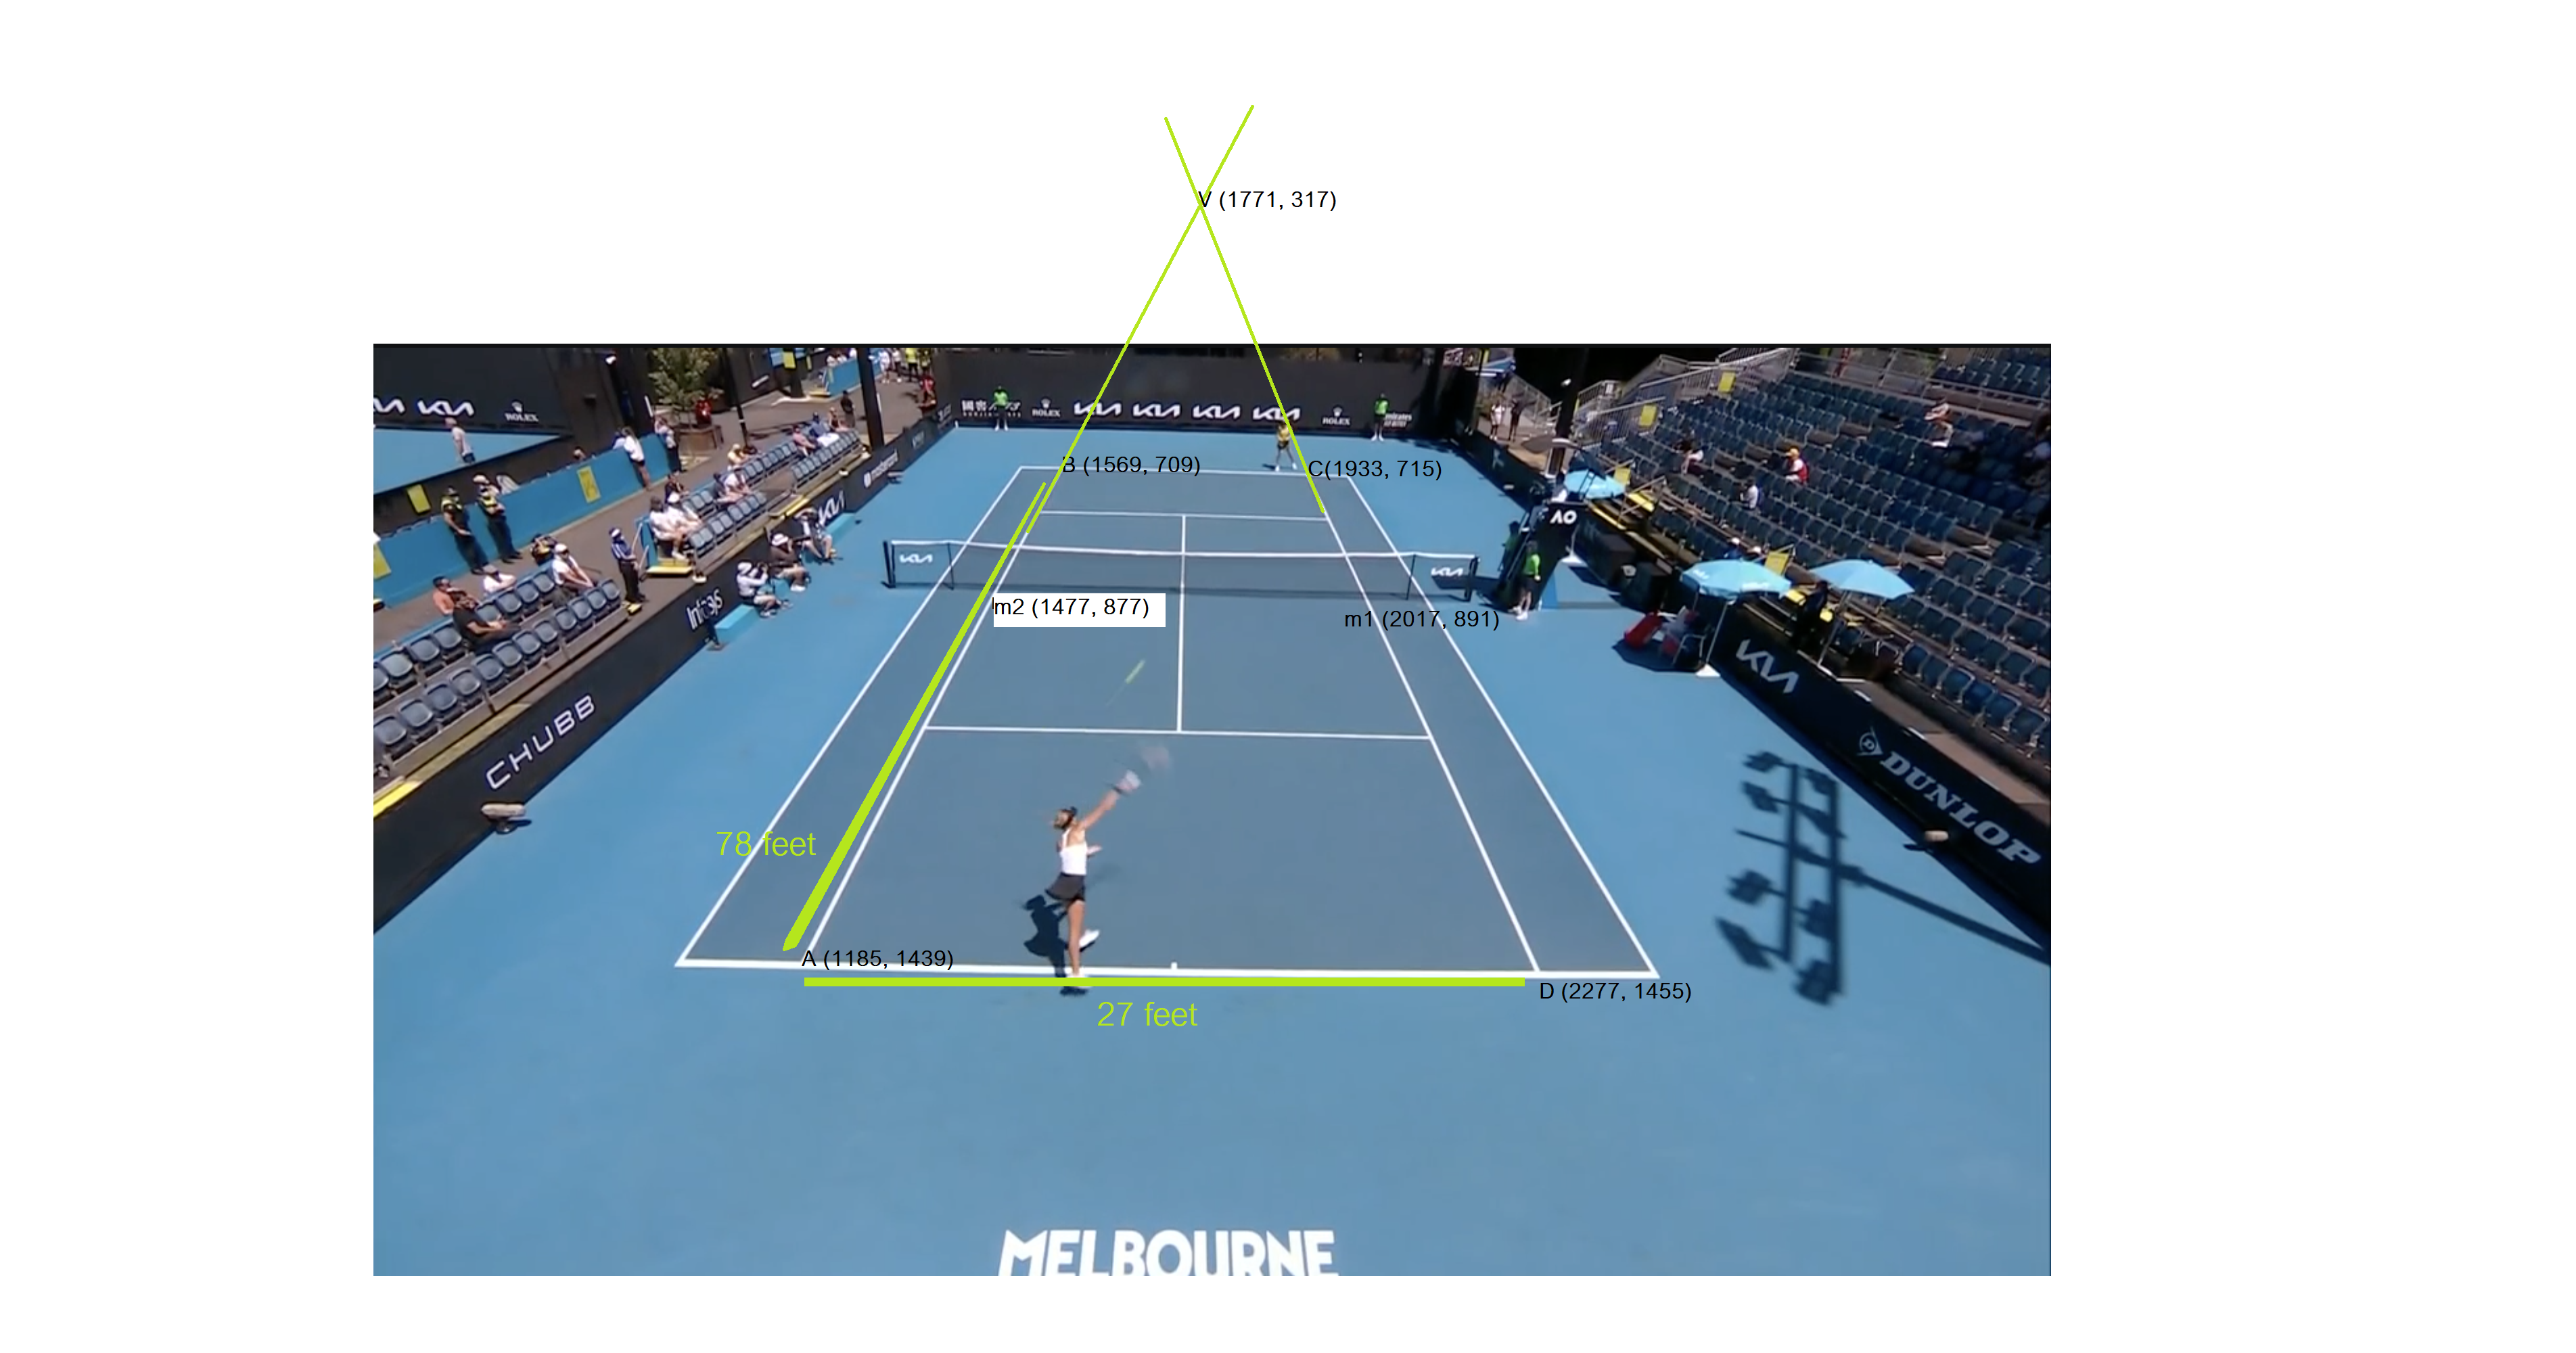
\includegraphics[width=0.475\textwidth]{imgs/tennis1}
  \hfill
  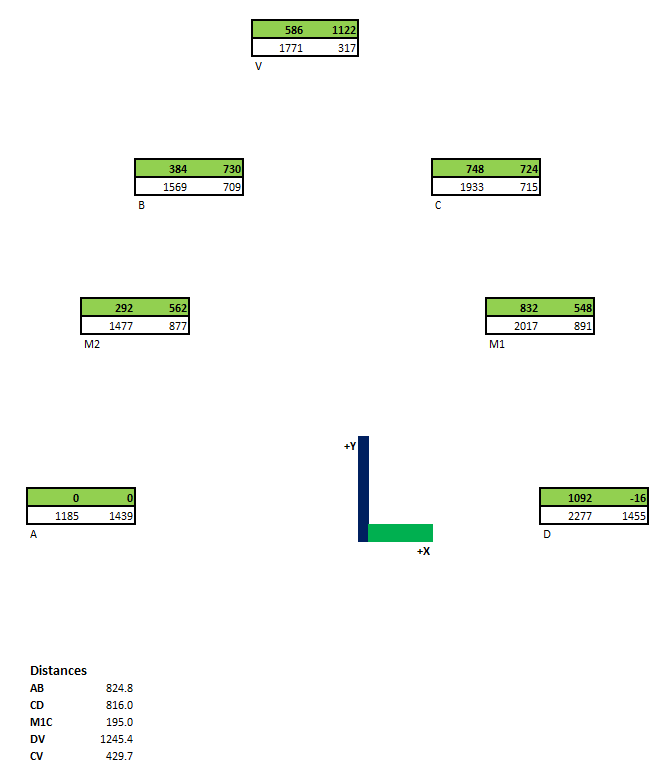
\includegraphics[width=0.475\textwidth]{imgs/tennis1_excel}
\end{figure}

\begin{figure}[H]
  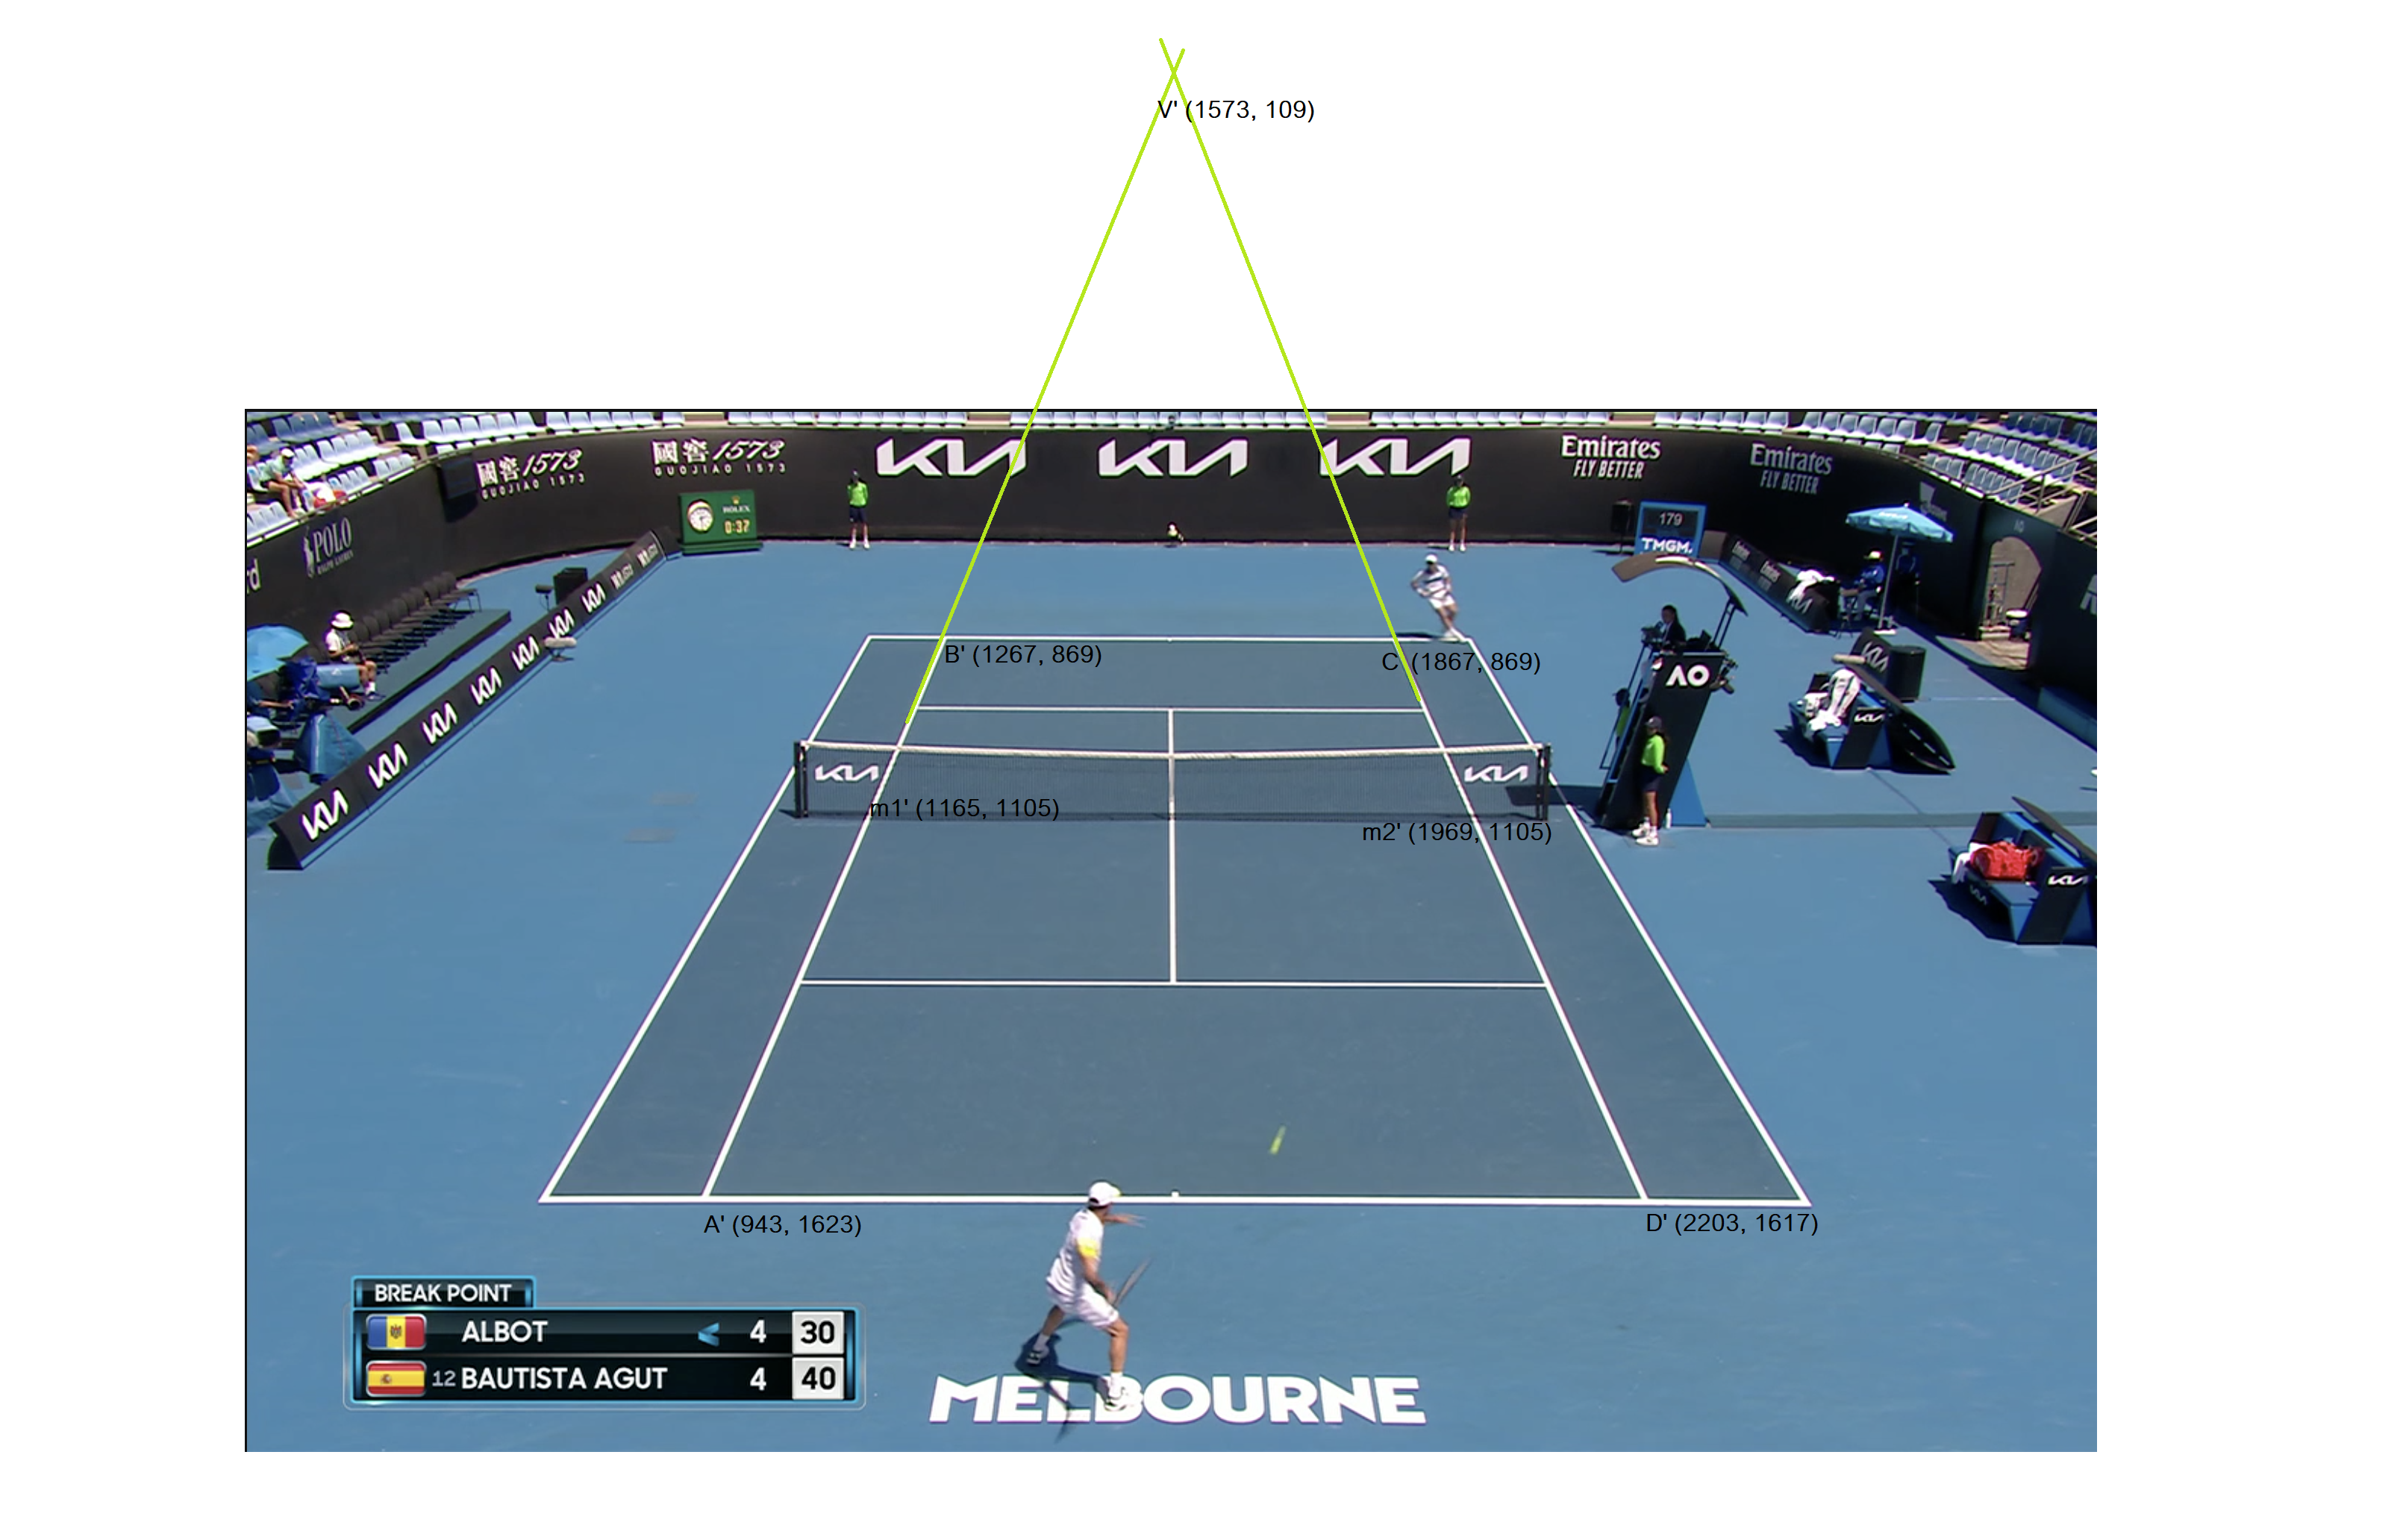
\includegraphics[width=0.475\textwidth]{imgs/tennis2}
  \hfill
  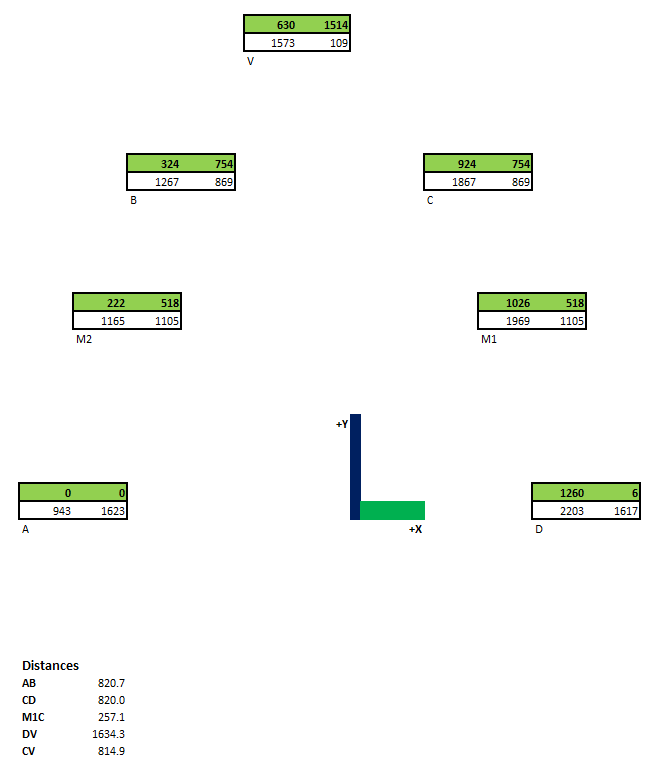
\includegraphics[width=0.475\textwidth]{imgs/tennis2_excel}
\end{figure}


\subsection{Find vanishing points using cross-ratios}

Known quantities:
\begin{table}[H]
\centering
\begin{tabular}{|c|c|l|}
\hline
\multicolumn{1}{|l|}{\textbf{Units}} & \textbf{Segment} & \textbf{Value}                \\ \hline
Image & $AD$      & $\sqrt{1092^2 + 16^2} = 1092$ pixels     \\ \hline
Image & $BC$      & $\sqrt{364^2 + 6^2} = 364$ pixels       \\ \hline
Image & $AB$      & $\sqrt{730^2 + 384^2} = 825$ pixels     \\ \hline
Image & $CD$      & $\sqrt{344^2 + 740^2} = 816$ pixels     \\ \hline
Image & $M_1 M_2$ & $\sqrt{540^2 + 14^2} = 540$ pixels     \\ \hline
Image & $A'D'$      & $\sqrt{1260^2 + 6^2} = 1260$ pixels     \\ \hline
Image & $B'C'$      & $\sqrt{600^2 + 0^2} = 600$ pixels       \\ \hline
Image & $A'B'$      & $\sqrt{324^2 + 754^2} = 821$ pixels     \\ \hline
Image & $C'D'$      & $\sqrt{336^2 + 748^2} = 820$ pixels     \\ \hline
Image & $M_1' M_2'$ & $\sqrt{804^2 + 0^2} = 804$ pixels     \\ \hline
World & $AD, A'D'$      & 27 feet     \\ \hline
World & $BC, B'C$       & 27 feet     \\ \hline
World & $AB, A'B'$      & 78 feet     \\ \hline
World & $CD, C'D'$      & 78 feet     \\ \hline
\end{tabular}
\end{table}

\textbf{Vanishing Point for Image 1}
\begin{align*}
  \frac{DC/DV}{{M_1}C/M_1V} &= \frac{C_wD_w/D_wV_w}{{M_1}_wC_w/{M_1}_wV_w} \\
  \frac{816/DV}{195/M_1V}                 &= 2 \cdot {M_1}_wV_w/D_wV_w \\
  \frac{816}{195}\cdot \frac{M_1V}{DV}    &= 2 \cdot {M_1}_wV_w/D_wV_w \\
  \frac{195 + CV}{816 + CV}   &= \frac{195}{816}\cdot 2 \cdot 1 \\
  (195 + CV) \cdot 816   &= 390 \cdot (816 + CV) \\
  CV \cdot (816 - 390)   &= 816 \cdot (390 - 195)\\
  CV  &= \frac{816 \cdot 195} {426}\\
  CV  &= 374\\
\end{align*}

Given the slope of the line and the distance $CV$, we can compute $V$ as follows:
\begin{align}
    m &= \frac{548-724}{832-748} = \frac{724-V_y}{748 - V_x}  \\
    374 &= \sqrt{(724-V_y)^2 + (748 - V_x)^2}
\end{align}

Solving the above system of equations using Mathematica, we obtain the possible
vanishing points as:
\begin{align*}
    {V_x\to 909.093,V_y\to 386.472} \\
    {V_x\to 586.907,V_y\to 1061.53} 
\end{align*}

Double-checking the answer using cross-products:

\textbf{Image 1 Vertical Vanishing Point}

\begin{align*}
L_1 &=    \begin{bmatrix}
            748 \\
            724 \\
            1
        \end{bmatrix} \times 
        \begin{bmatrix}
            1092 \\
            -16 \\
            1
        \end{bmatrix}  = 
        \begin{bmatrix}
            724 + 16 \\
            1092 - 748 \\
            -16*748 - 724*1092
        \end{bmatrix} = 
        \begin{bmatrix}
            740  \\
            344 \\
            -802576 
        \end{bmatrix}                                                   
\end{align*}

\begin{align*}
L_2 &=    \begin{bmatrix}
            384 \\
            730 \\
            1
        \end{bmatrix} \times 
        \begin{bmatrix}
            0 \\
            0 \\
            1
        \end{bmatrix}  = 
        \begin{bmatrix}
            730  \\
            -384 \\
            0 
        \end{bmatrix}                                                   
\end{align*}

Now, computing $L_1 \times L_2$ to obtain the vanishing point:
\begin{align*}
    \begin{bmatrix}
        740  \\
        344 \\
        -802576 
    \end{bmatrix} \times 
    \begin{bmatrix}
        730  \\
        -384 \\
        0 
    \end{bmatrix}   = 
\begin{bmatrix}
    576  \\
    1095 \\
    1 
\end{bmatrix}
\end{align*}

\textbf{Vanishing Point for Image 2}
\begin{align*}
  \frac{D'C'/D'V'}{{M_1}'C'/{M_1}'V'} &= \frac{{C_w}'{D_w}'/{D_w}'{V_w}'}
                                        {{{M_1}_w}'{C_w}'/{{M_1}_w}'{V_w}'} \\
  \frac{820/DV}{257/M_1V}                 &= 2 \cdot {M_1}_wV_w/D_wV_w \\
  \frac{820}{257}\cdot \frac{M_1V}{DV}    &= 2 \cdot {M_1}_wV_w/D_wV_w \\
  \frac{257 + CV}{820 + CV}   &= \frac{257}{820}\cdot 2 \cdot 1 \\
  (257 + CV) \cdot 820   &= 514 \cdot (820 + CV) \\
  CV \cdot (820 - 514)   &= 820 \cdot (514 - 257)\\
  CV  &= \frac{820 \cdot 257} {306}\\
  CV  &= 689\\
\end{align*}

Given the slope of the line and the distance $CV$, we can compute $V$ as follows:
\begin{align}
    m &= \frac{518-754}{1026-924} = \frac{754-V_y}{924 - V_x}  \\
    689 &= \sqrt{(754-V_y)^2 + (924 - V_x)^2}
\end{align}

Solving the above system of equations using Mathematica, we obtain the possible
vanishing points as:
\begin{align*}
    {V_x\to 1197.35,V_y\to 121.544} \\
    {V_x\to 650.65,V_y\to 1386.46} 
\end{align*}

\subsection{Find vanishing points for court baselines}

\subsubsection*{Image 1 Horizontal Vanishing Point}

\begin{align*}
L_1 &=    \begin{bmatrix}
            384 \\
            730 \\
            1
        \end{bmatrix} \times 
        \begin{bmatrix}
            748 \\
            724 \\
            1
        \end{bmatrix}  = 
        \begin{bmatrix}
            6  \\
            364 \\
            -268024 
        \end{bmatrix}                                                   
\end{align*}

\begin{align*}
L_2 &=    \begin{bmatrix}
            0 \\
            0 \\
            1
        \end{bmatrix} \times 
        \begin{bmatrix}
            1092 \\
            -16 \\
            1
        \end{bmatrix}  = 
        \begin{bmatrix}
            16  \\
            1092 \\
            0 
        \end{bmatrix}                                                   
\end{align*}

Now, computing $L_1 \times L_2$ to obtain the vanishing point:
\begin{align*}
    \begin{bmatrix}
        6  \\
        364 \\
        -268024 
    \end{bmatrix}     \times 
    \begin{bmatrix}
        16  \\
        1092 \\
        0 
    \end{bmatrix}    = 
    \begin{bmatrix}
        402036  \\
        -5891 \\
        1 
    \end{bmatrix}
\end{align*}


\subsubsection*{Image 2 Horizontal Vanishing Point}

\begin{align*}
    L_1 &=    \begin{bmatrix}
                324 \\
                754 \\
                1
            \end{bmatrix} \times 
            \begin{bmatrix}
                924 \\
                754 \\
                1
            \end{bmatrix}  = 
            \begin{bmatrix}
                0  \\
                600 \\
                -452400 
            \end{bmatrix}                                                   
    \end{align*}
    
    \begin{align*}
    L_2 &=    \begin{bmatrix}
                0 \\
                0 \\
                1
            \end{bmatrix} \times 
            \begin{bmatrix}
                1260 \\
                6 \\
                1
            \end{bmatrix}  = 
            \begin{bmatrix}
                -6  \\
                1260 \\
                0 
            \end{bmatrix}                                                   
    \end{align*}
    
    Now, computing $L_1 \times L_2$ to obtain the vanishing point:
    \begin{align*}
        \begin{bmatrix}
            0  \\
            600 \\
            -452400 
        \end{bmatrix}    \times 
        \begin{bmatrix}
            -6  \\
            1260 \\
            0 
        \end{bmatrix}    = 
        \begin{bmatrix}
            158340  \\
            754 \\
            1 
        \end{bmatrix}
    \end{align*}
    
\subsubsection*{Finding the homography that maps tennis court to 
                image plane}

\subsubsection*{Image 1} 

\begin{align*}
  W' \sim P
   \begin{bmatrix}
  0   \\
  0   \\
  1  
  \end{bmatrix} \implies 
  \alpha W' = P
   \begin{bmatrix}
  0   \\
  0   \\
  1  
  \end{bmatrix}   \\
  X' \sim P
   \begin{bmatrix}
  0   \\
  1   \\
  0  
  \end{bmatrix} \implies 
  \beta X' = P
   \begin{bmatrix}
  0   \\
  1   \\
  0  
  \end{bmatrix}  \\
  Y' \sim P
   \begin{bmatrix}
  1   \\
  0   \\
  0  
  \end{bmatrix} \implies 
  \gamma Y' = P
   \begin{bmatrix}
  1   \\
  0   \\
  0  
  \end{bmatrix}   \\
  Z' \sim P
   \begin{bmatrix}
  1   \\
  1   \\
  1  
  \end{bmatrix} \implies 
  \delta Z' = P
   \begin{bmatrix}
  27   \\
  78   \\
  1  
  \end{bmatrix} 
  \end{align*}
  
  Combining the above equations:
  \begin{align*}
  \delta Z' &= \alpha W' + \beta X' + \gamma Y' \\ \\
  \delta  \begin{bmatrix}
  1   \\
  1   \\
  1  
  \end{bmatrix}  &= \alpha  \begin{bmatrix}
  3  \\
  0   \\
  1  
  \end{bmatrix} +
  \beta \begin{bmatrix}
  0   \\
  3   \\
  1  
  \end{bmatrix} + \gamma  \begin{bmatrix}
  -3   \\
  0   \\
  1  
  \end{bmatrix} 
  \end{align*} 
  We can infer that $\delta = 1$, and simplify the system of equations to:
  \begin{align*}
  \begin{bmatrix}
  \alpha & \beta & \gamma
  \end{bmatrix}  &= \left(\begin{bmatrix}
  3 & 0 & -3   \\
  0 & 3  & 0  \\
  1 & 1  & 1	
  \end{bmatrix} \right) ^{-1}
  \begin{bmatrix}
  1  \\
  1   \\
  1  
  \end{bmatrix}
  \end{align*} 
  
  Solving for the inverse of the coefficient matrix, we obtain:
  \begin{align*}
  \begin{bmatrix}
  \frac{1}{6} & -\frac{1}{6} & \frac{1}{2}	\\
  0 & \frac{1}{3} & 0  \\
  -\frac{1}{6}  & -\frac{1}{6}  & \frac{1}{2}	
  \end{bmatrix} \implies 
  \begin{bmatrix}
  \alpha \\
  \beta \\
  \gamma
  \end{bmatrix} = 
  \begin{bmatrix}
  \frac{1}{2} \\
  \frac{1}{3} \\
  \frac{1}{6}
  \end{bmatrix} 
  \end{align*}
  
  From this, we obtain the transformation $P$ by multiplying $\alpha, \beta$ and $\gamma$ into the above equation:
  \begin{align*}
  \begin{bmatrix}
  \frac{3}{2} & 0 & -\frac{1}{2}	\\
  0 & 1 & 0  \\
  \frac{1}{2}  & \frac{1}{3}  & \frac{1}{6}	
  \end{bmatrix}
  \end{align*}
  
\subsection{Compute the focal length of each image}
\subsection{Compute the vanishing points using intersection of parallel lines}

\end{document}

